\section{Recap on fast KDE}
\subsection{What have I done before?}
\begin{frame}{Fast KDE}
\begin{block}{To find the outliers...}
Data points are scattered in "some" space, e.g., Euclidean space, Hilbert space.
Outliers are those points with lower density, which can be measured by Kernel Density Estimation (\textit{KDE}).
\end{block}
\begin{columns}
\hskip10pt
\begin{column}{.35\textwidth}
\begin{figure}
\centering
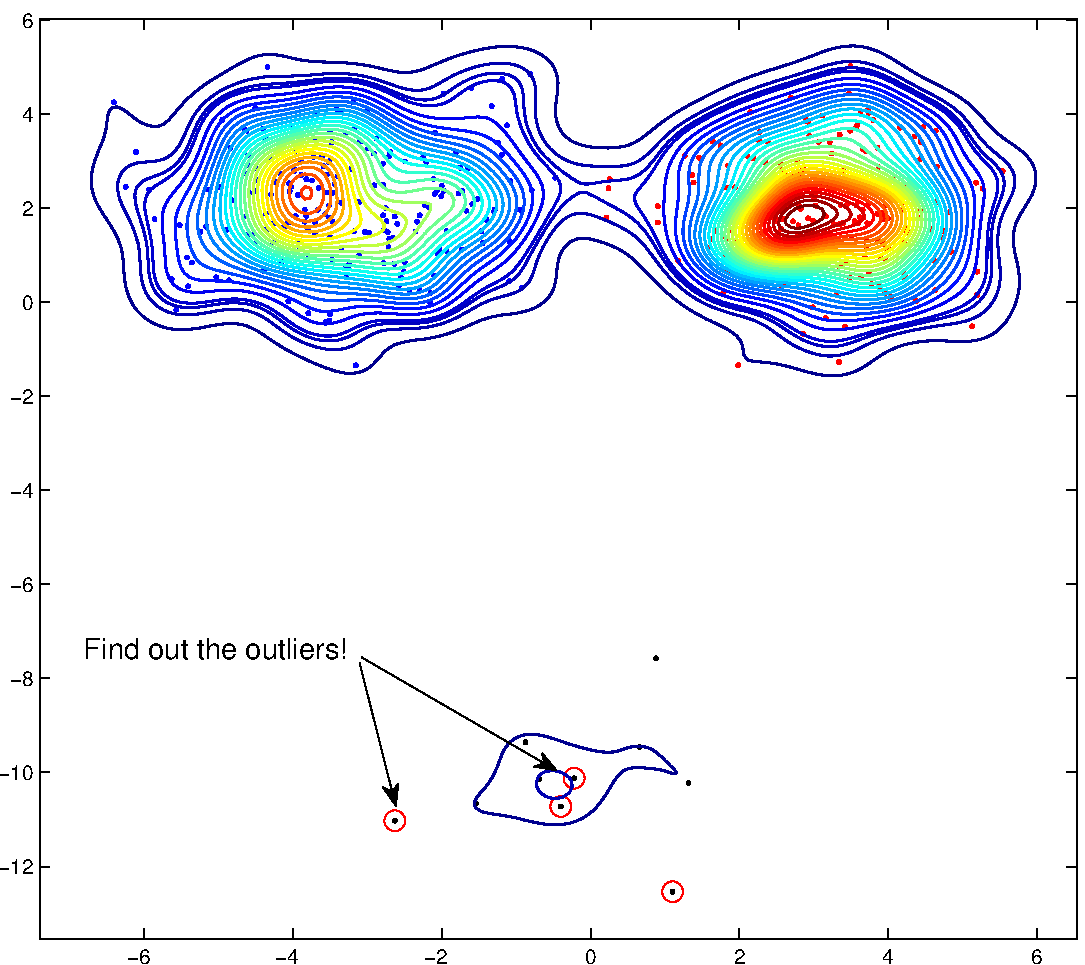
\includegraphics[scale=0.25]{imgs/outliers_density}
\end{figure}
\end{column}
\begin{column}{.65\textwidth}
\begin{center}
\small
The kernel density estimate of $x^*$ is
\[
f(x^*) = \frac{1}{nh}\sum^n_{i=1}K(\frac{x^* - x_i}{h})
\]
\color{red} Testing density is too much overhead!
\end{center}	
\end{column}
\end{columns}
\end{frame}


\begin{frame}{Fast KDE: use clustering}
\begin{flushleft}
Clustering the data points first
\end{flushleft}
\begin{columns}
\hskip10pt
\begin{column}{.35\textwidth}
\begin{figure}
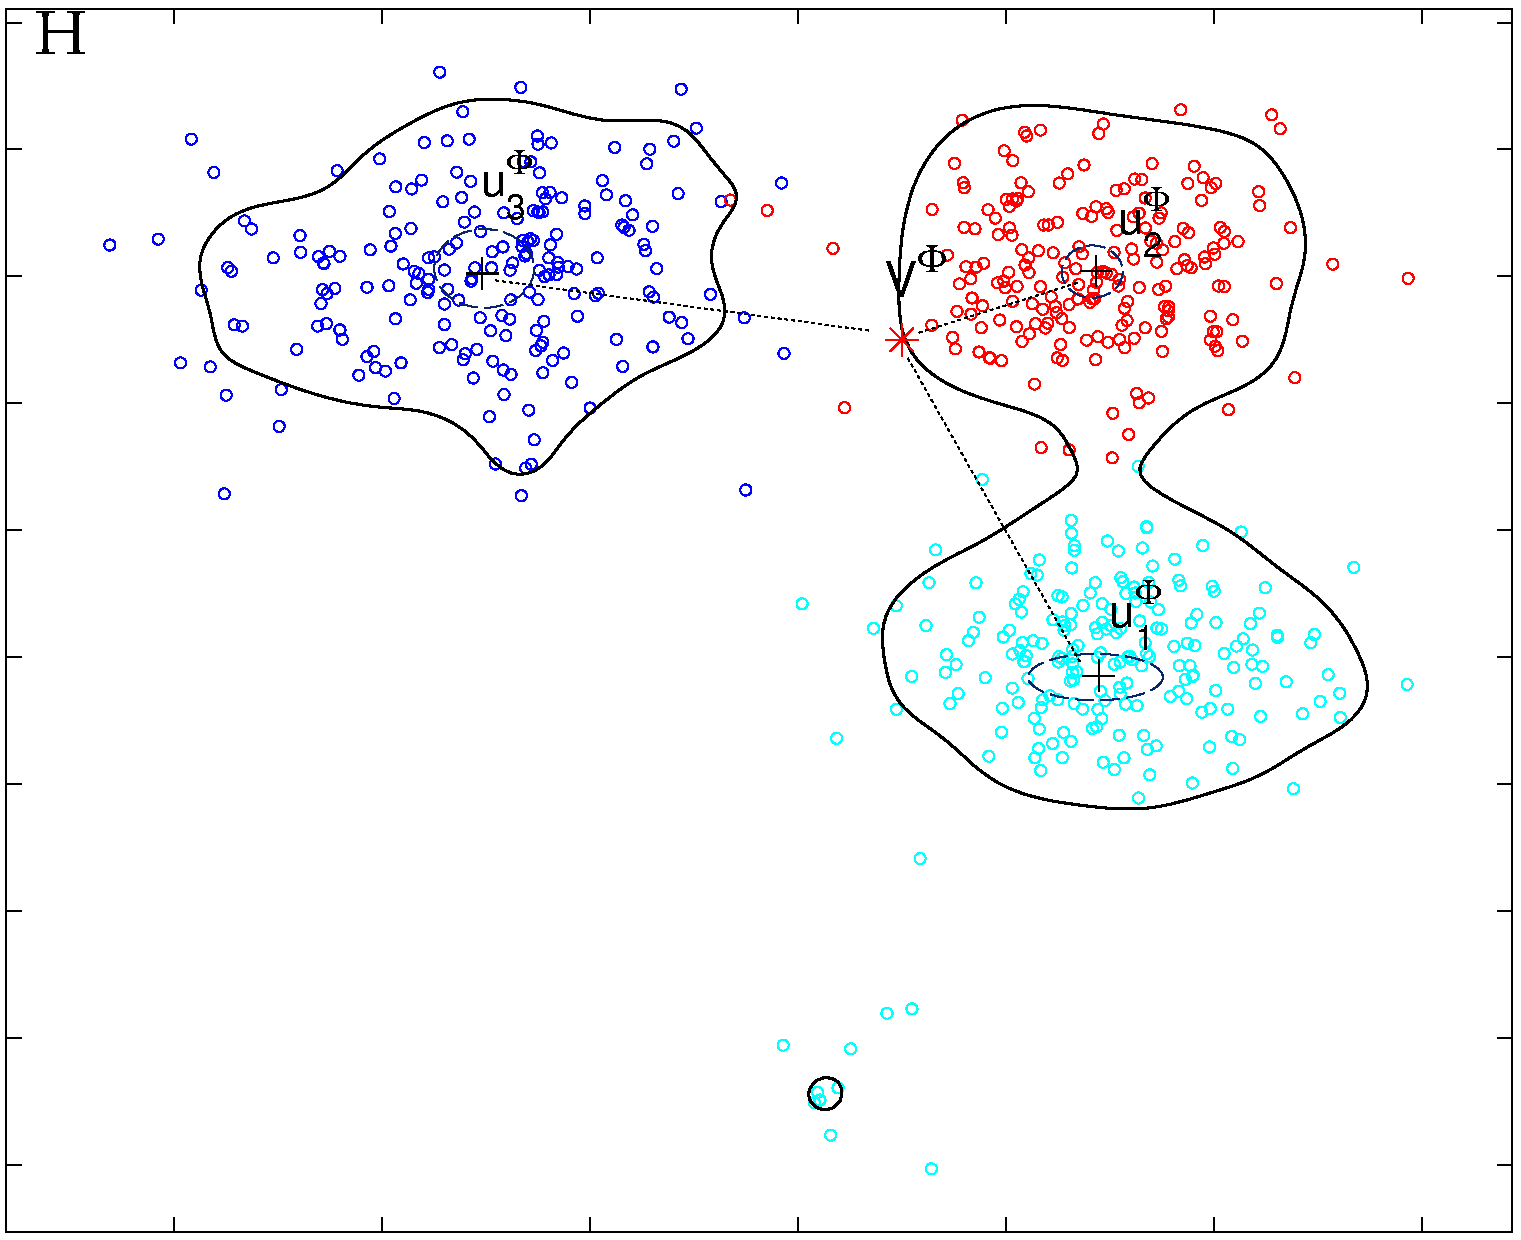
\includegraphics[width=3.5cm, height=3.5cm]{imgs/kclust}
\end{figure}
\end{column}
\begin{column}{.65\textwidth}
\small
\centering
Averaging on $m$ cluster centers:
\[
\hat{V}^\Phi=\frac{1}{m}\sum_{i=1}^m w_i\Phi_i(x_s)
\]
which is more efficient.\\ \vskip20pt \pause
\alert{BUT, lose too much precision, when $m$ is small}
\end{column}
\end{columns}
\end{frame}


\subsection{Compromised too much?}
\begin{frame}{Problems}
\begin{itemize}
\item Density approximation only rely on cluster centers.
\item Require to define how many clusters we have, i.e., $m=?$
\item Outliers are averaged equally, not robust.
\item We also need to integrate user feedback.
\end{itemize}
\end{frame}

\begin{frame}{Another clustering?}
\begin{block}{Solution}
Instead of looking for the cluster center, we look for the cluster bounds using support vectors. 
\end{block}
\end{frame}
%\begin{frame}{Causal Inference Overview}
%\begin{figure}
%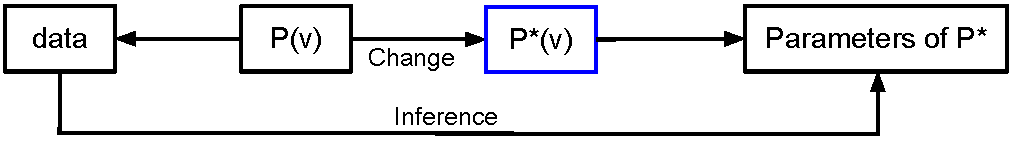
\includegraphics[scale=0.6]{imgs/causalInf}
%\end{figure}
%\begin{itemize}
%\item What if $P$ has shifted itself to $P^*$?
%\item<2-> \textbf{Key factors:} Causes, Changes, and Invariants . 
%\item<2-> Inference of $P^*$ and reasoning of changes. 
%\end{itemize}
%\end{frame}
%\begin{frame}{What makes Causal Inference interesting?}
%\begin{itemize}
%\item Human understands the world in terms of causes and effects.
%\item Empirical science is about establishing causes.
%\item Causal inference gives a mathematical language for causal
%statements, and tools to solve causal problems formally.
%\item Alternative exercising to decision making, reasoning, etc.
%\end{itemize}
%%\begin{alertblock}{Note}
%%Causal Inference has fundamental difference with machine learning
%%\end{alertblock}
%\end{frame}
%\subsection{Causal Graphical Model}
%\begin{frame}{Association}
%\begin{itemize}
%\item Now we want to find out what \alert{causes} lung cancer
%\end{itemize} \pause
%\begin{columns}
%\begin{column}{0.5\textwidth}
%\begin{table}
%\centering
%\begin{tabular}{|c|c|c|c|}
%\hline
%& & \multicolumn{2}{|c|}{Lung cancer}\\\hline
%smoking & yellow teeth & yes & no\\\hline
%yes & yes & 100 & 400\\\hline
%yes & no & 100 & 400\\\hline
%no & yes & 1 & 450\\\hline
%no & no & 9 & 8540\\\hline
%\end{tabular}
%\caption{Data observations from 10000 people}
%\end{table}
%\end{column}\hfill
%\begin{column}{0.5\textwidth}
%\vspace*{-0.5in}
%\begin{figure}
%\centering
%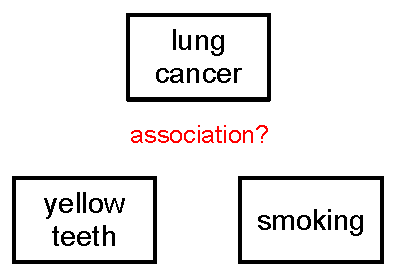
\includegraphics[scale=0.6]{imgs/smokepl}
%\end{figure}
%\end{column}
%\end{columns}
%\end{frame}
%\begin{frame}{Measurements of Association}
%\textbf{To find out associations among variables}
%\begin{itemize}
%\item Mutual information (Information theory)
%\item Pearson (linear) correlation
%\item Spearman's rho (rank correlation)
%\item Effect size between two variables
%\item Many others
%\end{itemize}
%\end{frame}
%\begin{frame}{Observations from Data}
%\textbf{Obviously}
%\begin{itemize}
%\item \textit{yellow teeth} and \textit{lung cancer} are associated.
%\end{itemize}\pause
%\alert{\textbf{But...}}
%\begin{itemize}
%\item Bleaching the teeth does not help reduce the probability
%of getting lung cancer.
%\end{itemize}\pause
%\begin{alertblock}{Caution!}
%Correlation does not imply Causation
%\end{alertblock}
%\end{frame}
%\begin{frame}{Statistical Implication}
%\begin{block}{Reichenbach's \textit{Common Cause Principle}}
%If $X$ and $Y$ are correlated, then either $X$ causes $Y$ or $Y$ causes $X$ or they share a latent common cause $Z$.
%\end{block}
%\begin{figure}
%\setcounter{subfigure}{0}
%	\centering
%	\begin{subfigure}[H]{0.3\textwidth}
%		\centering
%		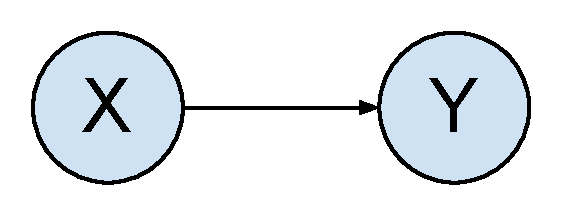
\includegraphics[scale=0.3]{imgs/x2y}
%		\caption{$X$ causes $Y$}
%		%\label{}	
%	\end{subfigure}
%	\begin{subfigure}[H]{0.3\textwidth}
%		\centering
%		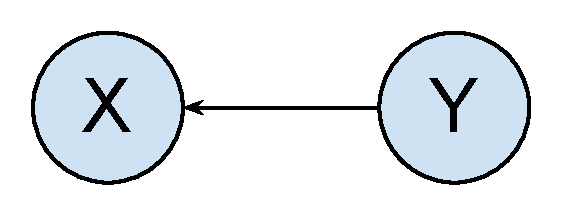
\includegraphics[scale=0.3]{imgs/y2x}
%		\caption{$Y$ causes $X$}
%		%\label{}	
%	\end{subfigure}
%	\begin{subfigure}[H]{0.3\textwidth}
%		\centering
%		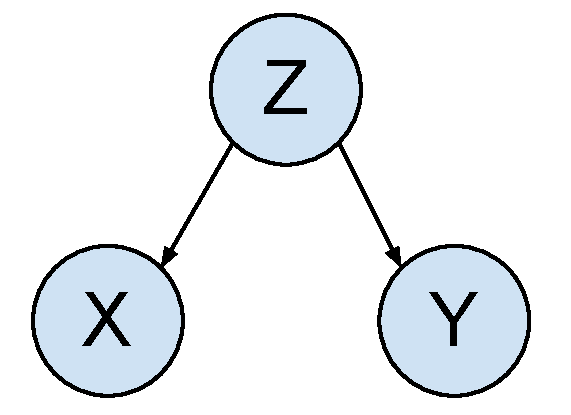
\includegraphics[scale=0.3]{imgs/z2xy}
%		\caption{A common latent cause $Z$}
%		%\label{}	
%	\end{subfigure}
%\end{figure}\pause
%\begin{itemize}
%\item<+-|alert@+> It links causality with probability
%\end{itemize}
%\end{frame}
%\begin{frame}{Functional Causal Model (pearl et al.)} 
%\begin{itemize}[<+->]
%\item A set of variables (factors) $\left\lbrace X_1,\ldots,X_n \right\rbrace$
%\item Directed acyclic graph $\mathcal{G}$ with vertices $\left\lbrace X_1,\ldots,X_n \right\rbrace$
%\item Parents of node $X_i$ in $\mathcal{G}$ are its direct causes
%\item $X_i=f_i(Parents(X_i),\epsilon_i)$, where $\left\lbrace\epsilon_1,\ldots,\epsilon_n\right\rbrace$ are jointly independent noises
%\item The above entails a joint probability distribution $P(X_1,\ldots,X_n)$
%\item Problems are twofold:
%      \begin{enumerate}
%		\item How is the $P$ like?
%		\item Can we recover $\mathcal{G} from P$? 
%	\end{enumerate}
%\item[] \begin{textblock*}{200mm}(0.6\textwidth,-2cm)
%		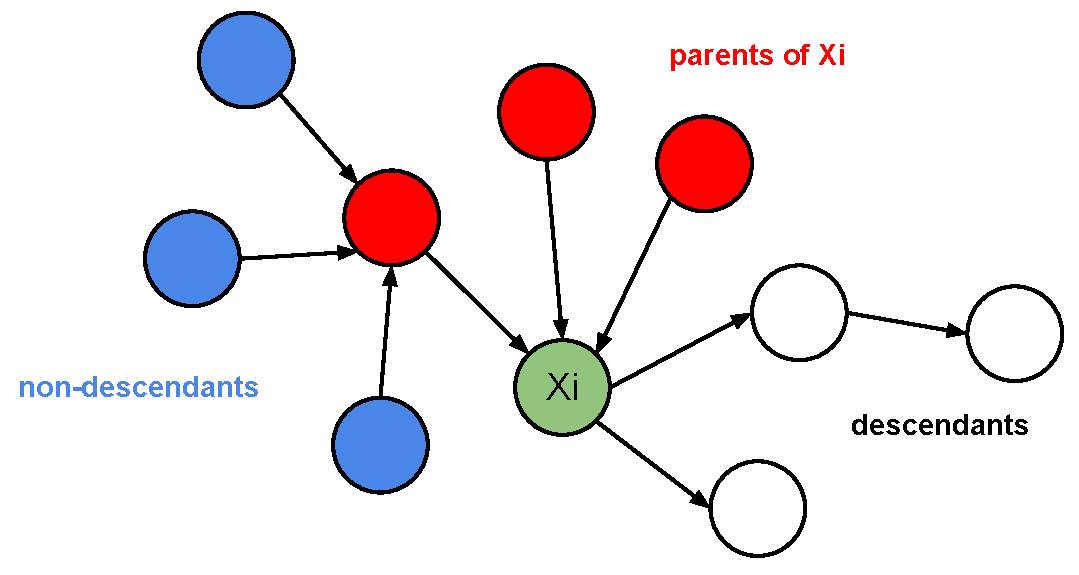
\includegraphics[scale=0.25]{imgs/causalgm}
%	\end{textblock*}
%\end{itemize}
%\end{frame}
%\begin{frame}{Functional Causal Model, ctd.}
%The following are equivalent:
%\begin{itemize}
%\item A functional causal model exists
%\item Local causal Markov condition: $X_i$ is statistically independent of its non-descendants given $X_i$'s parents
%\item Global Causal Markov condition: \textbf{d-separation} characterize the set of independences over all the observables
%\item Factorization: $P(X_1,\ldots,X_n)=\prod_iP(X_i\,|\,Parents(X_i))$
%\end{itemize}
%\end{frame}
%\begin{frame}{Learning causation from Data?}
%\begin{block}{Question}
%Given observational data, can we infer $\mathcal{G}$?
%\end{block}
%\begin{itemize}
%\item \textbf{Simple answer:} impossible without additional information
%\item Possible with interventions (outside force, empirical treatment, etc.)
%\item By conditional independence tests, \textit{Markov equivalence class} containing $\mathcal{G}$ can be learned. \alert{But}, it fails in simplest 2-nodes case.
%\item 2-nodes case can be tackled applying residual dependence test. (see Hoyer et al.)
%\end{itemize}
%\end{frame}
%\begin{frame}{Markov Equivalence Class}
%\textbf{Simplest case with three variables}
%\begin{itemize}
%\item[]<1-> \begin{figure}
%\setcounter{subfigure}{0}
%			\begin{subfigure}[H]{0.4\textwidth}
%			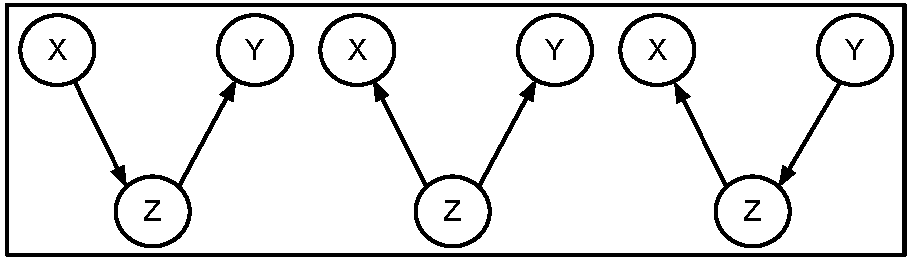
\includegraphics[scale=0.4]{imgs/eqv}
%			\caption{Equivalence}
%			\end{subfigure}\hfill
%			\begin{subfigure}[H]{0.3\textwidth}
%			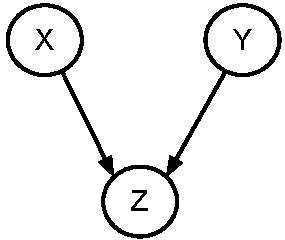
\includegraphics[scale=0.4]{imgs/noneqv}
%			\caption{Non-equivalence}
%			\end{subfigure}
%		\end{figure}
%\item<2-> Samples can be explained by all graphs in equivalence class
%\item<3-> For example:
%\begin{table}
%\centering
%\begin{tabular}{|c|c|}
%\hline
%Equivalence class & Non-equivalence class \\\hline
%$Dep(X,Z\,|\,\emptyset)$ & $Dep(X,Z\,|\,\emptyset)$\\\hline
%$Dep(Y,Z\,|\,\emptyset)$ & $Dep(Y,Z\,|\,\emptyset)$\\\hline
%$Dep(X,Y\,|\,\emptyset)$ & \alert{$Ind(X,Y\,|\,\emptyset)$}\\\hline
%$Ind(X,Y\,|\,Z)$ & \alert{$Dep(X,Y\,|\,Z)$}\\\hline
%\end{tabular}
%\end{table}	
%\end{itemize}
%\end{frame}